%!TEX root = ../../../root.tex

We have tried to define convolution in terms of one of its defining properties (a property that the convolution and only the convolution satisfies), i.e. translation invariance. We have seen how this is not possible since the very notion of translation is ill-defined in manifolds.

\paragraph{Convolution in the Fourier domain}

Therefore, we now try to define convolution in terms of another one of its defining properties, in particular the \emph{convolution theorem}. The convolution theorem states that the convolution is \emph{diagonalized} by the \emph{Fourier transform}, meaning that the Fourier transform of the convolution of two functions is simply the product of their Fourier transforms.
\begin{equation}
    \widehat{\left( f \star g \right)} = \hat{f} \cdot \hat{g}
\end{equation}

This is a first step, but simply transfers the problem, since a convolution involves a convolution integral (or sum) that in turn requires a Euclidean domain, but also the Fourier transform requires a similar integral (see \cref{sec:appendix:fourier} for a more in depth discourse on the Fourier transform). However, there is another mathematical object that comes to our rescue: the \emph{Laplacian} operator $\Delta$.

\paragraph{The connection with the Laplacian}
The Laplacian operator is naturally defined in the Euclidean domain as a differential operator, but can be generalized also to other domains, including graphs and meshes. 

\begin{figure}[H]
    \centering
    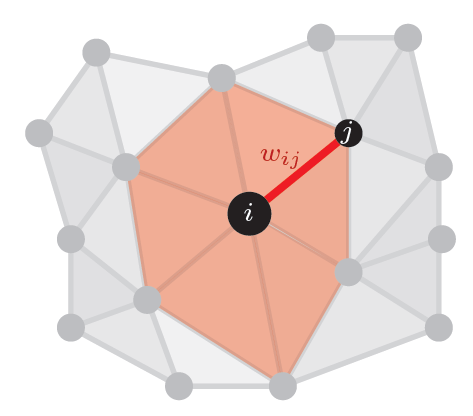
\includegraphics[width=.4\textwidth]{figures/12/laplacian.png}
    \caption{Neighborhood of a vertex.}
\end{figure}

The Laplacian acts locally on the neighborhood of each vertex. This is something that we like, since enforces locality by definition. Given a node signal $\vb{x}$, i.e. a function that associates features to each node $i$, the Laplacian associates to each node $i$ the quantity
\begin{equation}
    (\Delta \vb{x})_i = \sum_j w_{ij} (\vb{x}_i - \vb{x}_j).
    \label{eq:12:4:2:graph-laplacian}
\end{equation}

The nice thing about the Laplacian, is that its \emph{eigenfunctions} in the Euclidean domain are exactly the plane waves that make up the Fourier basis. What this means is that it is
\begin{equation}
    \hat{f}(\xi) = \int_{\mathbb{R}} f(x) \underbrace{e^{-2\pi i x \xi}}_{\mathclap{\text{function of the Fourier basis}}} dx 
\end{equation}
but also
\begin{equation}
    \Delta \underbrace{\left(e^{-2\pi i x \xi}\right)}_{} = 4 \pi^2 |\xi|^2 \underbrace{\left(e^{-2\pi i x \xi}\right)}_{}.
\end{equation}
Since the Laplacian operator leaves the plane wave unchanged, it is a eigenfunction.

The fact that the Fourier basis of the Euclidean domain is composed by the Laplacian eigenfunctions allows us to generalize the Fourier transform to any non-Euclidean domain $\mathcal{X}$:
\begin{equation}
    \hat{f}(\xi) = \sum_{k \geq 1} \underbrace{\int_{\mathcal{X}} f(x) \phi_k(x) dx}_{\langle {f, \phi_k \rangle }_{L^2(\mathcal{X})}} 
    \label{eq:12:4:2:non-euclidean-fourier}
\end{equation}
where 
\begin{equation}
    \Delta \phi_k(x) = \overbrace{\lambda_k}^{\mathclap{\text{eigenvalue of the Laplacian}}} \underbrace{\phi_k(x)}_{\mathclap{\text{eigenfunction of the Laplacian}}},
\end{equation}
and 
\begin{equation}
    \inner{\cdot}{\cdot}_{L^2(\mathcal{X})}
\end{equation}
is the inner product defined on the functional (Hilbert) space of functions defined over the manifold $\mathcal{X}$. Just like the inner product of two vectors in vector spaces is the sum of the product of all their elements, the inner product of two functions in functional spaces is the ``sum'' (integral) of the product of all the values they take over the domain.

\begin{figure}[H]
    \centering
    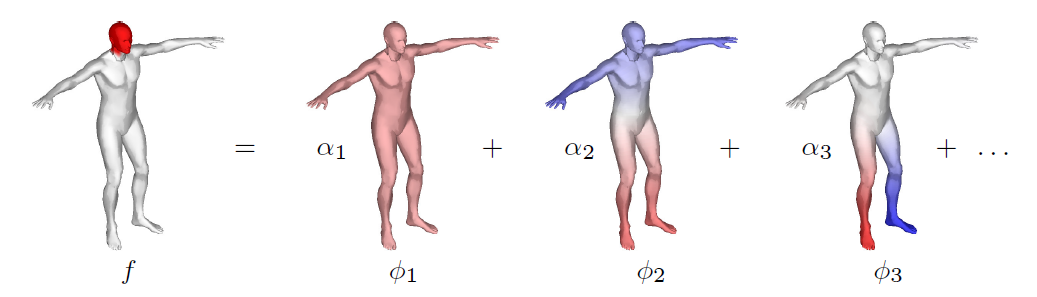
\includegraphics[width=.7\textwidth]{figures/12/fourier-basis-manifold.png}
    \caption{Decomposition of a function $f$ over a manifold (the mesh of a humanoid) as the terms of a Fourier series. The contributions of every eigenfunction $\phi_i$ of the Laplacian over the Manifold (Fourier basis), weighted by the appropriate eigenvalue $\alpha_1 = \hat{f}_i$ (Fourier coefficient) make up the original function $f$.}
\end{figure}

Now, we are able to express our node signal $f: \mathcal{X} \to \mathbb{R}$ defined on a non-Euclidean domain $\mathcal{X}$ in the Fourier (or spectral) domain, and perform convolution with a (spectral) filter in the Fourier domain as a simple product. 

\begin{align}
    (f \star g) (x) & = \sum_{k \geq 1} \inner{f}{\phi_k}_{L^2(\mathcal{X})} \underbrace{\inner{g}{\phi_k}_{L^2(\mathcal{X})}}_{} \phi_k (x) && \text{Fourier transform to obtain the spectral filter } \hat{g}_k \\
    & = \sum_{k \geq 1} \underbrace{\inner{f}{\phi_k}_{L^2(\mathcal{X})}}_{} \hat{g}_k \phi_k (x) && \text{Fourier transform to obtain } \hat{f}_k \\
    & = \sum_{k \geq 1} \underbrace{\hat{f}_k \hat{g}_k}_{} \phi_k (x) && \text{convolution as a product in the Fourier domain} \\
    & = \sum_{k \geq 1} \underbrace{\widehat{(f \star g)}_k \phi_k (x)}_{} && \text{inverse Fourier transform}.
\end{align}

\paragraph{Discrete spectral convolution}
Ok, but in practice we deal with discrete, not continuous objects. Our node signals does not vary continuously over the non-Euclidean domain $\mathcal{X}$, since this is actually a finite and discrete collection of nodes $\mathcal{V}$. Therefore the node signals are functions 
\begin{equation}
    f: \mathcal{V} \to \mathbb{R}
\end{equation}
encoded as vectors 
\begin{equation}
    \vb{f} = \mqty(f_{v_1}, f_{v_2}, \dots, f_{v_n})^{\top}
\end{equation}
that associate a scalar feature to each node $v \in \mathcal{V}$, with $|\mathcal{V}| = n$. 
\\

\textbf{Note.} If we had multiple features for each node, i.e. the node signal were multi-dimensional, i.e.
\begin{equation}
    f: \mathcal{V} \to \mathbb{R}^m
\end{equation}
then we would just encode this signal as a matrix
\begin{equation}
    \vb{F} = \mqty(
        \vb{f}_{v_1}^{\top} \\
        \vb{f}_{v_2}^{\top} \\
        \vdots \\
        \vb{f}_{v_n}^{\top}
    ) = \mqty(
        f_{v_1}^{(1)} & \dots & f_{v_1}^{(m)} \\
        f_{v_2}^{(1)} & \dots & f_{v_2}^{(m)} \\
        \vdots      & \ddots    & \vdots        \\
        f_{v_n}^{(1)} & \dots & f_{v_n}^{(m)} \\
    )
\end{equation}
that associates a $m$-dimensional vector feature to each node $v \in \mathcal{V}$, with $|\mathcal{V}| = n$. 
\\

In this setting the Laplacian is an operator $\Delta(\cdot)$ that when applied to a node signal $\vb{x}$, represented as a $n$-dimensional vector, returns a $n$-dimensional vector whose $i$-th component is defined as in \cref{eq:12:4:2:graph-laplacian}. Hence, it is a $(n \times n)$ matrix $\vb*{\Delta}$. Since it is a discrete object (a square matrix), we cannot talk about \emph{eigenfunctions}, but instead we deal with the more familiar \emph{eigenvectors}, that still share the fundamental property of being member of the Fourier basis in the non-Euclidean (now discrete) domain, for instance a graph. So we take an eigendecomposition of the Laplacian to yield
\begin{equation}
    \vb*{\Delta} = \vb*{\Phi} \vb*{\Lambda} \vb*{\Phi}^{\top},
\end{equation}
with 
\begin{equation}
    \vb*{\Phi} = \mqty(\vb*{\phi}_1, \dots, \vb*{\phi}_n)
\end{equation}
matrix of eigenvectors, and 
\begin{equation}
    \vb*{\Lambda} = \mathrm{diag} \{ \lambda_1, \dots, \lambda_n \}
\end{equation}
matrix of eigenvalues.

The Fourier transform \cref{eq:12:4:2:non-euclidean-fourier} now boils down to a simple matrix-vector product
\begin{equation}
    \begin{aligned}
        \hat{f}(\xi) = \hat{\vb{f}} & = \sum_{k \geq 1} \inner{\vb{f}}{\vb*{\phi}_k}_{L^2(\mathcal{X})} \\
        & = \sum_{k \geq 1} \vb{f}^{\top} \vb*{\phi}_k \\
        & = \sum_{k \geq 1} \vb*{\phi}_k^{\top} \vb{f}  \\
        & = \vb*{\Phi}^{\top} \vb{f}.
    \end{aligned}
\end{equation}
As you can imagine, the inverse Fourier transform will be the inverse $(\vb*{\Phi}^{\top})^{-1}$, but since it is always possible to perform an eigendecomposition in which the eigenvectors form an orthonormal eigenbasis, then we can assume $\vb*{\Phi}$ to be an orthogonal matrix, i.e. that it is 
\begin{equation}
    \vb*{\Phi}^{-1} = \vb*{\Phi}^{\top}   
\end{equation}
and therefore 
\begin{equation}
    (\vb*{\Phi}^{\top})^{-1} = (\vb*{\Phi}^{\top})^{\top} = \vb*{\Phi}.
\end{equation}
Therefore, the inverse Fourier transform will simply be 
\begin{equation}
    f(x) = \vb{f} = \vb*{\Phi} \hat{\vb{f}}.
\end{equation}

In this discrete setting, performing a spectral convolution of a node signal $f(x)$ encoded as a vector $\vb{f} = (f_1, \dots, f_n)^{\top}$ with a filter $g(x)$ encoded as a vector $\vb{g} = (g_1, \dots, g_n)^{\top}$ means
\begin{equation}
    \begin{aligned}
        \vb{f} \star \vb{g} & = \vb*{\Phi} \left[ \left(\vb*{\Phi}^{\top} \vb{g} \right) \odot \left(\vb*{\Phi}^{\top} \vb{f} \right) \right]\\
        & = \vb*{\Phi} \underbrace{\left( \hat{\vb{g}} \odot \hat{\vb{f}} \right)}_{\mathclap{\text{convolution as a (element-wise) product in the Fourier domain}}} \\ 
        & = \vb*{\Phi} \mqty( \hat{g}_1 \cdot \hat{f}_1 \\ \vdots \\ \hat{g}_n \cdot \hat{f}_n) \\
        & = \vb*{\Phi} \underbrace{\mqty(
            \hat{g}_1 & & \\
            & \ddots & \\
            & & \hat{g}_n
        )}_{\mathclap{\text{spectral filter}}} \mqty(\hat{f}_1 \\ \vdots \\ \hat{f}_n) \\ 
        & = \underbrace{\vb*{\Phi} \widehat{(f \star g)}}_{\mathclap{\text{inverse Fourier transform}}}.
        \label{eq:12:4:2:spectral-discrete-conv}
    \end{aligned}
\end{equation}

\paragraph{Limitations of the spectral convolution}

Is this newly defined convolution a proper convolution?

\subparagraph{The spectral convolution is not shift invariant}

One of the defining properties of convolution is shift invariance. Have we been able to recover this property, with this new approach? 

Recall that in the Euclidean (discrete) domain the shift invariance property of convolution comes from the peculiar structure of the matrix encoding the operation:
\begin{equation}
    \begin{aligned}
        \vb{f} \star \vb{g} & = \underbrace{\mqty(
            g_1 & g_2 & \dots & \dots & g_n \\
            g_n & g_1 & g_2 & \dots & g_{n-1} \\
            \vdots & \vdots & \ddots & \ddots & \vdots \\
            g_2 & g_3 & \dots & \dots & g_1
        )}_{\mathclap{\text{circulant matrix}}} ~ \vb{f}.
        \label{eq:12:4:2:circulant}
    \end{aligned}
\end{equation}

The fact that convolution in the Fourier domain is a simple product means that the Fourier basis (that as we have seen is composed by the Laplacian eigenvectors) \emph{diagonalizes} the circulant matrix:
\begin{equation}
    \mqty(
            g_1 & g_2 & \dots & \dots & g_n \\
            g_n & g_1 & g_2 & \dots & g_{n-1} \\
            \vdots & \vdots & \ddots & \ddots & \vdots \\
            g_2 & g_3 & \dots & \dots & g_1
        ) = \vb*{\Phi} \mqty(
            \hat{g}_1 & & \\
            & \ddots & \\
            & & \hat{g}_n
        ) \vb*{\Phi}^{\top} = \vb*{\Phi} ~ \mathrm{diag}\{ \hat{g}_1, \dots, \hat{g}_n \} ~ \vb*{\Phi}^{\top},
\end{equation}
and this is another way of seeing the derivation done in \cref{eq:12:4:2:spectral-discrete-conv}. However, for the spectral convolution we have defined to be shift invariant, we should be able to express it as a matrix-vector product in which the matrix has a circulant structure, as in \cref{eq:12:4:2:circulant}. But it turns out that in
\begin{equation}
    \begin{aligned}
        \vb{f} \star \vb{g} & = \underbrace{\vb*{\Phi} ~ \mathrm{diag}\{ \hat{g}_1, \dots, \hat{g}_n \} ~ \vb*{\Phi}^{\top}}_{\vb{G}} \vb{f} \\
        & = \vb{G} \vb{f}
    \end{aligned}
\end{equation}
the matrix $\vb{G}$ does \emph{not} have a circulant structure, so the spectral convolution is \emph{not} shift-invariant. 


\subparagraph{Spectral convolution is domain dependent}

Convolution is domain dependent. In fact, recall that the Fourier basis that allows us to generalize the Fourier transform to any domain, and so to perform the convolution, is composed by the eigenfunctions $\phi_1, \dots, \phi_n$ of the Laplacian, that \emph{depend on the domain}. 

This is true also with regular Euclidean convolution, in which the Fourier basis are the plane waves $e^{-2\pi i \vb{x}\cdot\vb*{\xi}}$. We never thought about this as a problem, since all our data, like images, live in the Euclidean domain $\mathbb{R}^n$, properly discretized to obtain images represented as pixels. 

However, in this new setting being domain dependent means that if we employed spectral convolution (as defined so far) in a model, composed by layers that would learn the proper spectral filters $\hat{\vb{g}}$ just like regular Euclidean convolutional layers would do, then this model would be intrinsecally bounded to that specific domain. Imagine the domain to be a graph. We have developed a very powerful model to perform some inference on the graph. Now, after training, we would like to test our model on a new, unseen graph. Well, the model is useless, since that is another, completely different domain, in which the Laplacian acts differently and hence has different eigenfunctions leading to different Fourier basis. The spectral convolution in this new domain is \emph{defined differently}, so the spectral filters we spent so much time learning at training time on a different graph are of no use here. 

\begin{figure}[H]
    \centering
    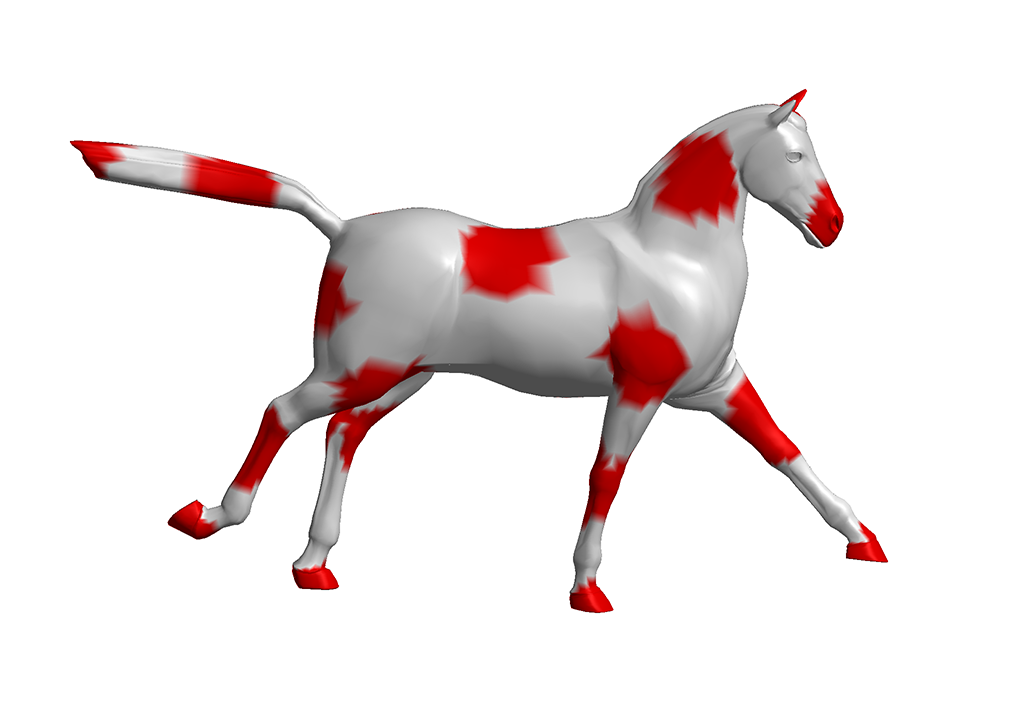
\includegraphics[width=.5\textwidth]{figures/12/horse0.png}
    \caption{Signal $\vb{x}$ over the horse's mesh.}
    \label{fig:12:4:2:horse-signal}
\end{figure}

Imagine this scenario, now on a mesh. We have trained our (spectral) CNN to ``detect edges'' of some node signal $\vb{x}$ (as you can see in \cref{fig:12:4:2:horse-signal}) on a mesh, for instance of a horse, and learned a spectral filter $\hat{\vb{Y}}$ so that on this mesh, that is one specific domain with its specific Fourier basis $\vb*{\Phi}$, the spectral convolution 
\begin{equation}
    \vb*{\Phi} \hat{\vb{Y}} \vb*{\Phi}^{\top} \vb{x}
\end{equation} 
seems to be producing nice results, as shown in \cref{fig:12:4:2:spectral-horse}.
\begin{figure}[H]
    \centering
    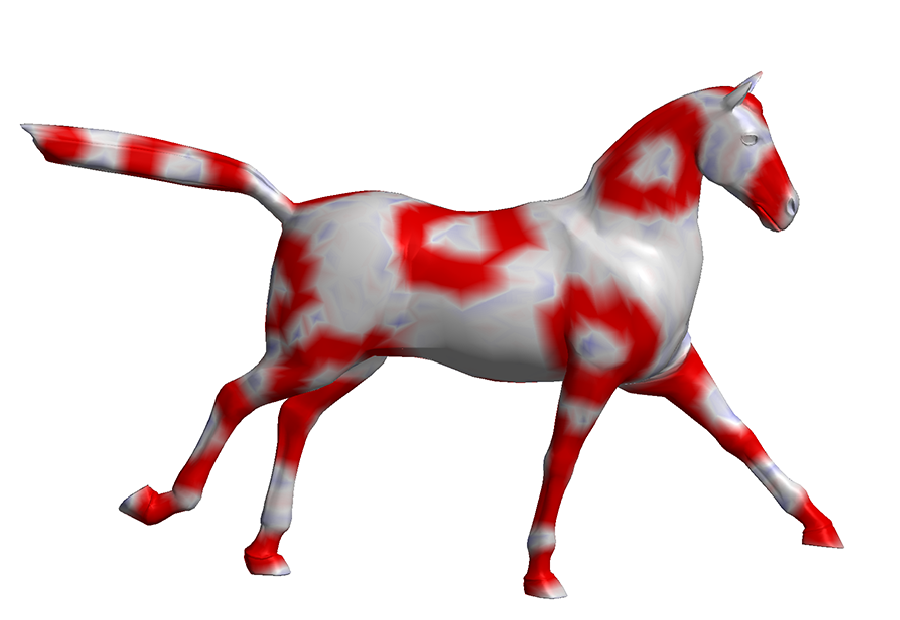
\includegraphics[width=.5\textwidth]{figures/12/spectral-horse.png}
    \caption{Edge detection on a mesh. }
    \label{fig:12:4:2:spectral-horse}
\end{figure}

So, we would imagine that our model was still able to detect edges if the mesh was animated, e.g. with the horse running, since our filter is now \emph{intrinsic}, it operates directly on the manifold and not on the embedding space and so it deforms with the mesh and therefore it should not be affected. However, at each frame the mesh deforms into a new mesh, that is a new domain with a new Fourier basis $\vb*{\Psi}$. Therefore, our edge detection model now computes
\begin{equation}
    \vb*{\Psi} \hat{\vb{Y}}  \vb*{\Psi}^{\top} \vb{x}
\end{equation}
since it has no choice, the very \emph{operation} of convolution is defined differently in this new domain, the model can only choose what spectral filters to use.

\begin{figure}[H]
    \centering
    \animategraphics[loop, autoplay, width=0.5\textwidth]{20}{12/animations/horse_edge/frame}{0}{22}
    \caption{As you can imagine, our nice edge detection model fails miserably}
\end{figure}

\subparagraph{Spectral convolution is not local}

As we have defined it, we have no guarantee that spectral convolution will be local in space. We can visualize spatially the learnt spectral filters
\begin{equation}
    \mathrm{diag} \{ \hat{g}_1, \dots, \hat{g}_n \}
\end{equation}
by going back to the spatial domain with an inverse Fourier transform
\begin{equation}
    \vb*{\Phi} \mathrm{diag} \{ \hat{g}_1, \dots, \hat{g}_n \}.
\end{equation}
When going back to the spatial domain, we see a spatial representation of the convolutional filters. Usually, these filters are not local at all, which instead is what we would like to have.

\paragraph{Variants of the spectral convolution}

Of course these are \emph{huge} limitations, and several works in recent years have tried to overcome them.

\subparagraph{Spectral CNN with smooth spectral filters}

This technique modifies the definition of spectral convolution to try and overcome the problem of non-locality. Instead of learning a spectral filter $\mathrm{diag} \{ \hat{g}_1, \dots, \hat{g}_n \}$ to perform the spectral convolution
\begin{equation}
    f \star g = \vb*{\Phi} ~ \mathrm{diag} \{ \hat{g}_1, \dots, \hat{g}_n \} ~ \vb*{\Phi}^{\top} \vb{f}
\end{equation}
as we have defined it so far, we now learn some \emph{smooth transformation} $\tau(\vb*{\Lambda})$ acting on the eigenvalues $\vb*{\Lambda}$ of the Laplacian. So the values $\hat{g}_1, \dots, \hat{g}_n$ cannot be arbitrary values, but must be the eigenvalues $\lambda_1, \dots, \lambda_n$ of the $\vb*{\Delta}$, transformed in some way. We want to learn this transformation.

Of course, if we allowed any transformation to be learned, then we would go back to having arbitrary values $\hat{g}_1, \dots, \hat{g}_n$. Instead, it turns out that by restricting the transformation $\tau(\cdot)$ to be \emph{smooth}, we obtain the \emph{localization in space} that we wanted.

This result is the \emph{Parseval's identity}, an important result in signal processing theory. In the standard Euclidean setting it states
\begin{equation}
    \int_{-\infty}^{+\infty} |x|^{2k} |f(x)|^2 dx = \int_{-\infty}^{+\infty} \left| \pdv[k]{\hat{f}(\omega)}{\omega} \right|^2.
\end{equation}
On the left hand side we have the spatial domain, in the spatial variable $x$. If the integral converges for a certain $k$, then this provides a measure of the \emph{locality} of the function in space.

On the right hand side we have the frequency (or spectral, or Fourier, they are all synonyms) domain, defined in terms of the \emph{angular frequency} variable $\omega = 2 \pi \xi$. If the integral converges for a certain $k$, then this provides a measure of the \emph{smoothness} of the function in frequency.

The two concepts are the same. So, extending this identity to the non-Euclidean setting, this means that if we want our filters $\tau(\vb*{\Lambda})$ to be localized in space, we must require $\tau(\cdot)$, that operates in frequency, to be smooth. 

We choose the transformation to be a \emph{linear combination of smooth functions}, in which the coefficients of the linear combination will be the \emph{learnable parameters}.
\begin{equation}
    \tau_{\vb*{\alpha}}(\lambda_k) = \sum_{j = 1}^{r} \alpha_j \beta_j (\lambda_k)
\end{equation}
in which $\vb*{\alpha} = (\alpha_1, \dots, \alpha_r)^{\top}$ is the vector of filter (learnable) parameters, and $\beta_1(\lambda), \dots, \beta_r(\lambda)$ are \emph{smooth kernel functions}. This works well since a linear combination of smooth functions is also a smooth function. Now, we can choose the various kernel functions to be any smooth functions (e.g. polynomials), and this choice becomes a hyperparameter of the model.

\begin{figure}[H]
    \centering
    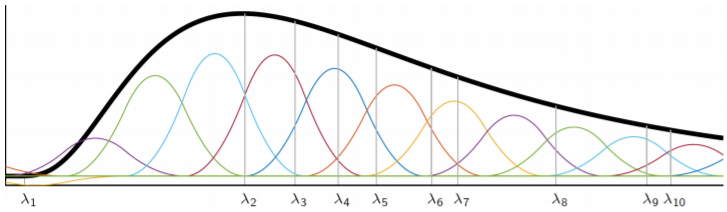
\includegraphics[width=.7\textwidth]{figures/12/40_46.png}
    \caption{Linear combination of $10$ Gaussian kernel functions, that yields a smooth transformation of the Laplacian eigenvalues. This will translate to a localized filter.}
\end{figure}

So we are parametrizing our spectral filter to be a smooth \emph{parametric} filter $\tau_{\vb*{\alpha}}(\cdot)$, so that the convolutional filter will operate to compute
\begin{equation}
    \begin{aligned}
        \vb{f} \star \vb{g} & = \vb*{\Phi} \underbrace{\mathrm{diag} \{ \hat{g}_1, \dots, \hat{g}_n \}}_{\tau_{\vb*{\alpha}}(\vb*{\Lambda})} \vb*{\Phi}^{\top} \vb{f}  \\
        & = \vb*{\Phi} \mqty(
            \tau_{\vb*{\alpha}}(\lambda_1) & & \\
            & \ddots & \\
            & & \tau_{\vb*{\alpha}}(\lambda_n)
        ) \vb*{\Phi}^{\top} \vb{f}
    \end{aligned}
    \label{eq:12:4:2:smooth-spectral-conv-1}
\end{equation}

If we write
\begin{equation}
    \tau_{\vb*{\alpha}}(\lambda_k) = \sum_{j = 1}^{r} \alpha_j \beta_j (\lambda_k) = (\vb{B} \vb*{\alpha})_k
\end{equation}
where $\vb{B}$ is a $(n \times r)$ matrix result by a column-by-column stacking of the $r$ smooth kernels $\beta$ defined on every one of $n$ eigenvalues, then we can write \cref{eq:12:4:2:smooth-spectral-conv-1} as 
\begin{equation}
    \vb*{\Phi} \mqty(
            (\vb{B} \vb*{\alpha})_1 & & \\
            & \ddots & \\
            & & (\vb{B} \vb*{\alpha})_n
        ) \vb*{\Phi}^{\top} \vb{f} = \vb*{\Phi} \vb{W} \vb*{\Phi}^{\top} \vb{f}
\end{equation}
where $\vb{W} = \mathrm{diag}(\vb{B} \vb*{\alpha})$ is the weight matrix of the layer, in which $\vb{B}$ is a fixed, domain-dependent transformation and $\vb*{\alpha}$ is the parameters to be learned. Recall that these are $r$ scalar values, so the number of parameters \emph{does not depend on the input size}, therefore we have $O(1)$ parameters per layer, similarly to the Euclidean convolution. In fact, we can think of $r$ as kernel size of a Euclidean convolutional filter. 
\\

\textbf{Note.} This technique manages to rescue locality, but the problem of domain independence still remains.